\section{Estudo com Redes de Bayes}
\label{sec:bayes}

\textbf{Redes de Bayes} é um modelo probabilístico que permite definir as relações de dependência entre determinadas variáveis e pode ser utilizado para calcular a probabilidade de ocorrência de determinados eventos associados a essas varáveis.

Ao pesquisarmos sobre outros estudos feitos de \textit{machine learning} sob o mesmo \textit{dataset} usado, encontramos a implementação \cite{kaggle_bayes}. Este utilizador do \textit{Kaggle} conseguiu, para 5 classes, obter uma precisão de aproximadamente $0.72$ e uma \textit{accuracy} de aproximadamente $0.61$ \footnote{Apesar do autor não ter documentado esta métrica, nós executamos o código disponibilizado pelo mesmo, obtendo este valor, para 10 mil \textit{features} (não podemos usar mais por falta de recursos físicos)} para os dados de teste.


\subsection{Repartição dos dados}
\label{subsub:bayes_data}

Para além da divisão descrita na secção \ref{subsub:data_initial_division}, fizemos uma segunda divisão nos dados reservados para treino/\textit{cross validation}. Esta divisão foi de realizada de maneira a que obtivéssemos uma distribuição de 60\%-20\%-20\% entre dados de treino, \textit{cross validation} e teste, respectivamente. A distribuição final dos dados por \textit{dataset} pode ser consultada nos gráficos da figura \ref{fig:data_distribution_with_cv}.

\begin{figure*}[!t]
	\centering
	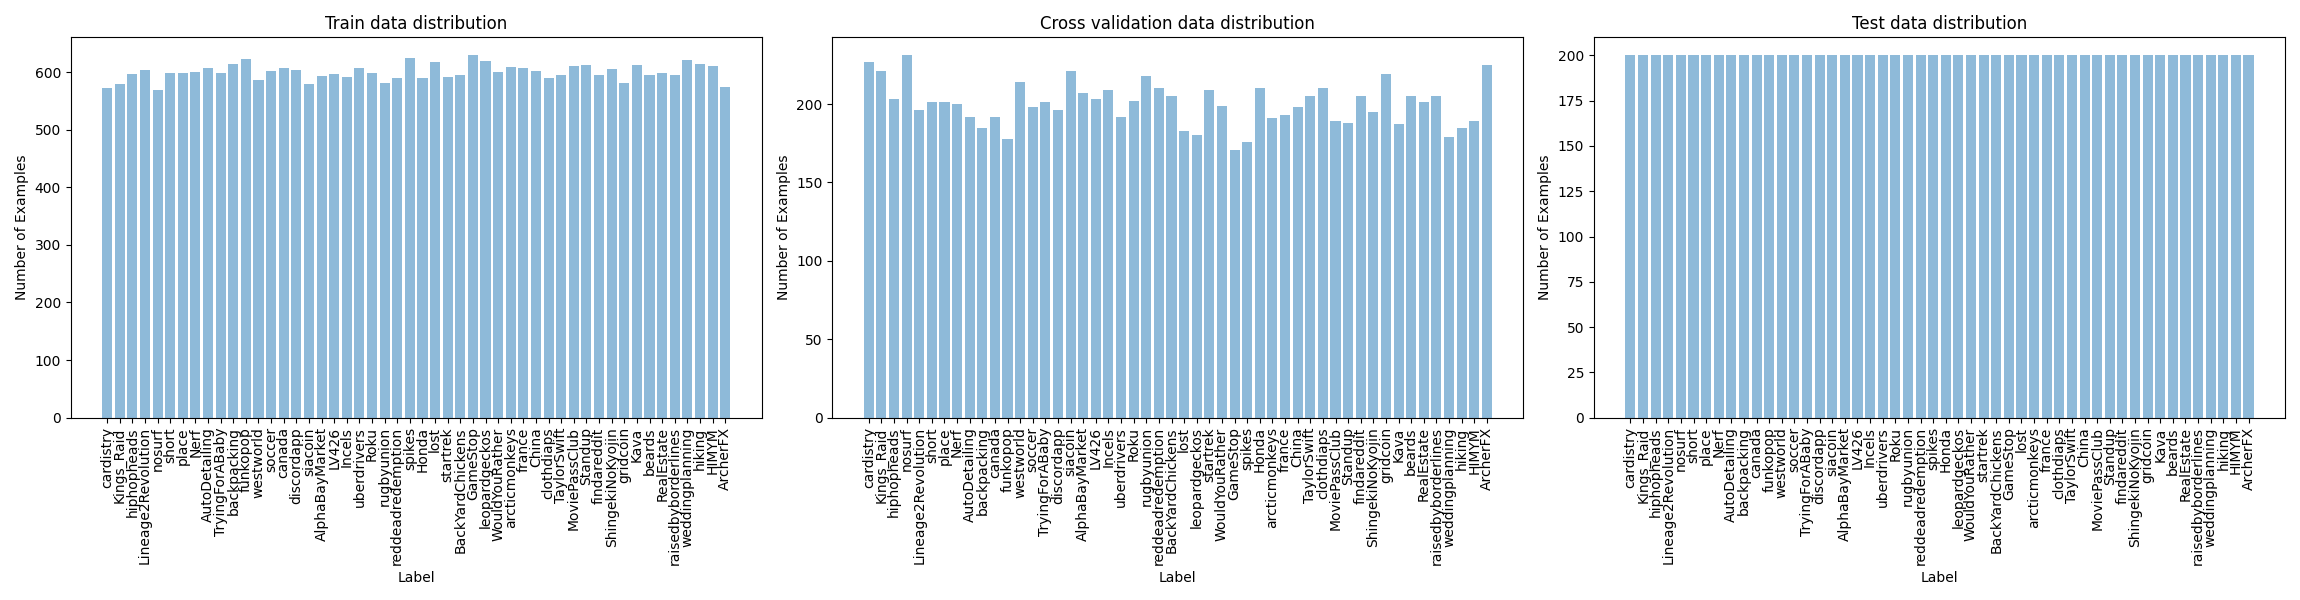
\includegraphics[width=\textwidth]{all_distribution_cv}
	\caption{Distribuição de dados por \textit{label} por \textit{dataset}, havendo discriminação entre dados de treino e de \textit{cross validation}.}
	\label{fig:data_distribution_with_cv}
\end{figure*}


\subsection{Resultados obtidos}
\label{sub:results_bayes}

Para obter os resultados que iremos descrever de seguida, adaptamos o código que encontramos no \textit{Kaggle} deste autor e fizemos algumas alterações de forma a usar a nossa técnica de extracção de \textit{features} dos dados, explicada na secção \ref{subsub:data_pre_processing}, ao invés da utilizada pelo autor. 

Desta forma, para 50 classes (ao invés das 5 usadas pelo autor original), obtivemos a variação de \textit{accuracy} de acordo com a variação do valor de alfa \footnote{\textit{Learning rate}} para os dados de treino e de \textit{cross validation} apresentados no gráfico da figura \ref{diagram:accuracy_alfa_bayes}. Como se pode verificar neste gráfico, foi obtido um valor máximo de $accuracy = 0.845$ para $\alpha = 0.1$ quando submetemos o modelo aos dados de \textit{cross validation}. 

\begin{figure}[t]
\begin{center}
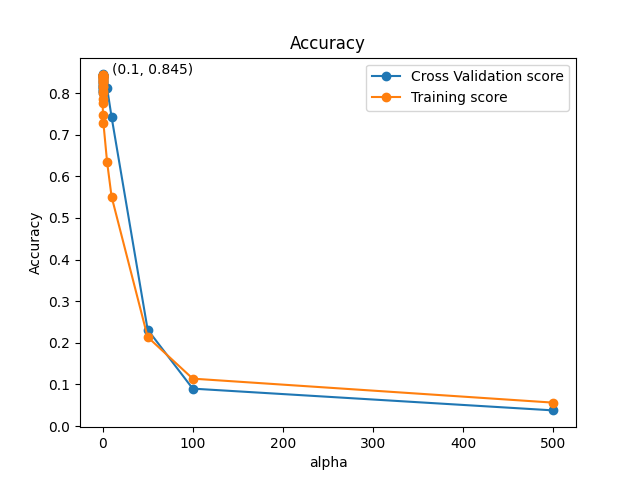
\includegraphics[width=0.5\textwidth,keepaspectratio]{figures/accuracy_alpha.png}
\caption{Gráfico da variação da \textit{accuracy} para valores de alfa entre $1*10^{-10}$ e $5*10^{2}$, para os dados de treino e de \textit{cross validation}}
\label{diagram:accuracy_alfa_bayes}
\centering
\end{center}
\end{figure}

O nosso passo seguinte foi retreinar o modelo onde obtivemos maior valor de alfa, usando como dados de treino os dados previamente usados para treino e \textit{cross validation}, ou seja, 80\% dos dados usados. Os resultados das métricas de performance por classe e totais quando o modelo foi treinado nas condições referidas podem ser consultados na tabela \ref{tab:bayes_perforamnce}. Duma forma geral, podemos verificar que temos resultados aceitáveis, mas não extraordinários (a \textit{accuracy} está longe de ser 100\%).

\begin{table}[!t]
\caption{Métricas de performance para $\alpha = 0.1$}
\begin{center}
\begin{tabular}{l c c c c}
Class & Accuracy & Recall & Precision & F1 Score\\ \hline
0 & 0.855 & 0.855 & 0.905 & 0.879\\
1 & 0.79 & 0.79 & 0.903 & 0.843\\
2 & 0.885 & 0.885 & 0.868 & 0.876\\
3 & 0.92 & 0.92 & 0.944 & 0.932\\
4 & 0.66 & 0.66 & 0.75 & 0.702\\
5 & 0.83 & 0.83 & 0.79 & 0.81\\
6 & 0.88 & 0.88 & 0.907 & 0.893\\
7 & 0.915 & 0.915 & 0.88 & 0.897\\
8 & 0.78 & 0.78 & 0.729 & 0.754\\
9 & 0.95 & 0.95 & 0.931 & 0.941\\
10 & 0.835 & 0.835 & 0.879 & 0.856\\
11 & 0.92 & 0.92 & 0.92 & 0.92\\
12 & 0.805 & 0.805 & 0.92 & 0.859\\
13 & 0.935 & 0.935 & 0.921 & 0.928\\
14 & 0.88 & 0.88 & 0.846 & 0.863\\
15 & 0.895 & 0.895 & 0.937 & 0.916\\
16 & 0.965 & 0.965 & 0.889 & 0.926\\
17 & 0.92 & 0.92 & 0.953 & 0.936\\
18 & 0.845 & 0.845 & 0.837 & 0.841\\
19 & 0.815 & 0.815 & 0.867 & 0.84\\
20 & 0.905 & 0.905 & 0.896 & 0.9\\
21 & 0.945 & 0.945 & 0.926 & 0.936\\
22 & 0.84 & 0.84 & 0.853 & 0.846\\
23 & 0.72 & 0.72 & 0.623 & 0.668\\
24 & 0.965 & 0.965 & 0.928 & 0.946\\
25 & 0.64 & 0.64 & 0.715 & 0.675\\
26 & 0.875 & 0.875 & 0.888 & 0.882\\
27 & 0.97 & 0.97 & 0.965 & 0.968\\
28 & 0.965 & 0.965 & 0.858 & 0.908\\
29 & 0.695 & 0.695 & 0.675 & 0.685\\
30 & 0.685 & 0.685 & 0.811 & 0.743\\
31 & 0.79 & 0.79 & 0.81 & 0.8\\
32 & 0.94 & 0.94 & 0.935 & 0.938\\
33 & 0.805 & 0.805 & 0.782 & 0.793\\
34 & 0.81 & 0.81 & 0.72 & 0.762\\
35 & 0.945 & 0.945 & 0.945 & 0.945\\
36 & 0.865 & 0.865 & 0.779 & 0.82\\
37 & 0.895 & 0.895 & 0.836 & 0.865\\
38 & 0.85 & 0.85 & 0.944 & 0.895\\
39 & 0.91 & 0.91 & 0.74 & 0.816\\
40 & 0.925 & 0.925 & 0.845 & 0.883\\
41 & 0.76 & 0.76 & 0.694 & 0.726\\
42 & 0.825 & 0.825 & 0.864 & 0.844\\
43 & 0.925 & 0.925 & 0.916 & 0.92\\
44 & 0.67 & 0.67 & 0.753 & 0.709\\
45 & 0.93 & 0.93 & 0.964 & 0.947\\
46 & 0.815 & 0.815 & 0.795 & 0.805\\
47 & 0.87 & 0.87 & 0.93 & 0.899\\
48 & 0.79 & 0.79 & 0.849 & 0.819\\
49 & 0.845 & 0.845 & 0.96 & 0.899\\
\hline
Macro Average & 0.853 & 0.853 & 0.856 & 0.853\\
\end{tabular}
\label{tab:bayes_perforamnce}
\end{center}
\end{table}


\subsection{Conclusão}

Apesar dos resultados finais obtidos terem sido aceitáveis, mas não extraordinários como demonstrado anteriormente, conseguimos obter um melhor valor de \textit{accuracy} que o autor da solução apresentada no inicio desta secção (aproximadamente $0.61$, para 5 classes, que ele obteve e $0.853$, para 50 classes, que nós obtivemos). Sendo que a maior alteração que fizemos à sua solução foi a utilização de um pré-processamento e selecção de \textit{features} distinta, concluímos que terá sido essa a chave para o nosso maior sucesso.
